\newpage
\def\thoigian{90}%--Thời gian
\de{Đề số 3}{Chương IV. Hệ thức lượng trong tam giác}
%[ID]%[Dự án D - Đợt 4 NH24-25 - Lê Hữu Kiệt]

\begin{center}
	\textbf{PHẦN 1 - CÂU TRẮC NGHIỆM BỐN PHƯƠNG ÁN}% 12 câu
\end{center}
\Opensolutionfile{ans}[ans/ans-TN-10-ONTAPCHUONG-IV-DE3]
\begin{ex}%[0H4N1-2]%[Dự án D - Đợt 4 NH24-25 - Lê Hữu Kiệt]
Trong các đẳng thức sau đây, đẳng thức nào đúng?
\choice
{$\sin150^\circ = -\dfrac{\sqrt3}{2}$}
{$\cos150^\circ = \dfrac{\sqrt3}{2}$}
{\True $\tan150^\circ = -\dfrac{1}{\sqrt3}$}
{$\cot150^\circ = \sqrt3$}
\loigiai{Ta có $\tan150^\circ = -\dfrac{1}{\sqrt3}$.}
\end{ex}

\begin{ex}%[0H4N1-2]%[Dự án D - Đợt 4 NH24-25 - Lê Hữu Kiệt]
Trên nửa đường tròn đơn vị cho điểm $M\left(-\dfrac{5}{13};\dfrac{12}{13}\right)$. Gọi $\alpha=\widehat{xOM}$, giá trị $\tan\alpha$ bằng
\choice
{$-\dfrac{5}{13}$}
{$-\dfrac{12}{13}$}
{$-\dfrac{5}{12}$}
{\True $-\dfrac{12}{5}$}
\loigiai{Theo định nghĩa, ta có $\tan\alpha=\dfrac{\dfrac{12}{13}}{-\dfrac{5}{13}}=-\dfrac{12}{5}$.\\
Vậy $\tan\alpha=-\dfrac{12}{5}$}
\end{ex}

\begin{ex}%[0H4N1-2]%[Dự án D - Đợt 4 NH24-25 - Lê Hữu Kiệt]
Cho góc $0^\circ\leq \alpha \leq 90^\circ$, trong các mệnh đề sau, mệnh đề nào là \textbf{sai}?
\choice
{$\sin(180^\circ-\alpha)=\sin\alpha$}
{\True $\cos(180^\circ-\alpha)=\cos\alpha$}
{$\sin(90^\circ-\alpha)=\cos\alpha$}
{$\cos(90^\circ-\alpha)=\sin\alpha$}
\loigiai{Với $0^\circ\leq \alpha \leq 90^\circ$ ta có
\begin{multicols}{2}
\begin{itemize}
	\item[] $\sin(180^\circ-\alpha)=\sin\alpha$.
	\item[] $\cos(180^\circ-\alpha)=-\cos\alpha$.
	\item[] $\sin(90^\circ-\alpha)=\cos\alpha$.
	\item[] $\cos(90^\circ-\alpha)=\sin\alpha$.
\end{itemize}
\end{multicols}
Vậy mệnh đề sai là $\cos(180^\circ-\alpha)=\cos\alpha$.
}
\end{ex}

\begin{ex}%[0H4N1-3]%[Dự án D - Đợt 4 NH24-25 - Lê Hữu Kiệt]
Cho góc $\alpha$ thỏa $0^\circ \leq \alpha \leq 180^\circ$. Giá trị của biểu thức $K=\sin(180^\circ-\alpha)+\sin\alpha$ bằng
\choice
{\True $2\sin\alpha$}
{$0$}
{$\sin180^\circ$}
{$1$}
\loigiai{Ta có $\sin(180^\circ-\alpha)=\sin\alpha$ với $0^\circ \leq \alpha \leq 180^\circ$.\\
Khi đó $K=\sin(180^\circ-\alpha)+\sin\alpha=\sin\alpha+\sin\alpha=2\sin\alpha$.\\
Vậy $K=2\sin\alpha$.}
\end{ex}

\begin{ex}%[0H4N2-1]%[Dự án D - Đợt 4 NH24-25 - Lê Hữu Kiệt]
Cho tam giác $ABC$ có $AB=2$, $AC=1$ và $\widehat{A}=60^\circ$. Tính độ dài cạnh $BC$.
\choice
{$BC=\sqrt2$}
{$BC=1$}
{\True $BC=\sqrt3$}
{$BC=2$}
\loigiai{
Theo định lý côsin ta có
\begin{eqnarray*}
	BC = \sqrt{AB^2 + AC^2 - 2AB\cdot AC\cdot \cos60^\circ}=\sqrt{2^2 + 1^2 - 2\cdot2\cdot1\cdot\dfrac{1}{2}} = \sqrt3.
\end{eqnarray*}
Vậy $BC=\sqrt3$.
}
\end{ex}

\begin{ex}%[0H4N2-1]%[Dự án D - Đợt 4 NH24-25 - Lê Hữu Kiệt]
Cho tam giác $ABC$ nội tiếp đường tròn $(O;R)$. Đẳng thức nào sau đây là đúng?
\choice
	{$BC = 2R\cos A$}
	{\True $BC = 2R\sin A$}
	{$BC = 2R\tan A$}
	{$BC = R\sin A$}
\loigiai{Do $\triangle ABC$ nội tiếp đường tròn $(O;R)$ nên theo định lí sin ta có
$$\dfrac{BC}{\sin A}=\dfrac{CA}{\sin B}=\dfrac{AB}{\sin C}=2R.$$
Suy ra $BC=2R\sin A$.
}
\end{ex}

\begin{ex}%[0H4N2-1]%[Dự án D - Đợt 4 NH24-25 - Lê Hữu Kiệt]
Cho tam giác $ABC$ có $AB=5$, $\widehat{A}=40^\circ$, $\widehat{B}=60^\circ$. Độ dài $BC$ gần nhất với kết quả nào nhất?
\choice
{$3{,}7$}
{\True $3{,}3$}
{$3{,}5$}
{$3{,}1$}
\loigiai{
Ta có $\widehat{C}=180^\circ - \widehat{A} - \widehat{B} = 180^\circ - 40^\circ - 60^\circ = 80^\circ$. \\
Áp dụng định lý sin ta ta $\dfrac{BC}{\sin A} = \dfrac{AB}{\sin C}$ suy ra $BC = \dfrac{AB\sin A}{\sin C} = \dfrac{5\sin 40^\circ}{\sin 80^\circ} \approx 3{,}3$.\\
Vậy độ dài $BC$ gần nhất với kết quả $3{,}3$.
}
\end{ex}

\begin{ex}%[0H4N2-1]%[Dự án D - Đợt 4 NH24-25 - Lê Hữu Kiệt]
Cho tam giác $ABC$ có $AB=5$ cm, $BC=5$ cm, $AC=3$ cm. Giá trị $\cos A$ là
\choice
{$-\dfrac{2}{3}$}
{$\dfrac{1}{2}$}
{\True $\dfrac{3}{10}$}
{$-\dfrac{3}{10}$}
\loigiai{Áp dụng hệ quả định lí hàm số côsin ta có
$$\cos A = \dfrac{AB^2+AC^2-BC^2}{2\cdot AB\cdot AC}=\dfrac{5^2+3^2-5^2}{2\cdot5\cdot3}=\dfrac{3}{10}.$$\\
Vậy $\cos A=\dfrac{3}{10}$.}
\end{ex}

\begin{ex}%[0H4N2-1]%[Dự án D - Đợt 4 NH24-25 - Lê Hữu Kiệt]
Cho tam giác $ABC$ có $BC=a$, $\widehat{BAC}=120^\circ$. Bán kính đường tròn ngoại tiếp $ABC$ là
\choice
{$R=a$}
{$R=\dfrac{a\sqrt{3}}{2}$}
{$R=\dfrac{a}{2}$}
{\True $R=\dfrac{a\sqrt{3}}{3}$}
\loigiai{
Áp dụng định lí sin ta có $\dfrac{BC}{\sin\widehat{BAC}}=2R$.\\
Suy ra $R=\dfrac{BC}{2\sin\widehat{BAC}}=\dfrac{a}{2\sin120^\circ}=\dfrac{a\sqrt3}{3}$.\\
Vậy bán kính đường tròn ngoại tiếp $ABC$ là $R=\dfrac{a\sqrt3}{3}$.
}
\end{ex}

\begin{ex}%[0H4H2-1]%[Dự án D - Đợt 4 NH24-25 - Lê Hữu Kiệt]
Cho tam giác $ABC$ có $BC=a$, $CA=b$, $AB=c$ thoả mãn hệ thức $b+c=2a$. Trong các mệnh đề sau, mệnh đề nào đúng?
\choice
{$\cos B+\cos C=2\cos A$}
{\True $\sin B+\sin C=2\sin A$}
{$\sin B+\sin C=\dfrac{1}{2}\sin A$}
{$\sin B+\cos C=2\sin A$}
\loigiai{
Theo định lý sin ta có $\dfrac{a}{\sin A} = \dfrac{b}{\sin B} = \dfrac{c}{\sin C}$. \\
Áp dụng dãy tỉ số bằng nhau, suy ra
$$\dfrac{a}{\sin A} = \dfrac{b}{\sin B} = \dfrac{c}{\sin C}=\dfrac{b+c}{\sin B+\sin C}=\dfrac{2a}{\sin B+\sin C}.$$
Khi đó $\dfrac{a}{\sin A}=\dfrac{2a}{\sin B + \sin C}$, suy ra $\sin B + \sin C = 2\sin A$.
}
\end{ex}

\begin{ex}%[0H4N2-2]%[Dự án D - Đợt 4 NH24-25 - Lê Hữu Kiệt]
Cho tam giác $ABC$ có $BC=4$ cm, $CA=6$ cm, $AB=8$ cm. Khi đó diện tích của tam giác $ABC$ bằng
\choice
{$9\sqrt{15}$ cm$^2$}
{\True $3\sqrt{15}$}
{$105$ cm$^2$}
{$\dfrac{2}{3}\sqrt{15}$ cm$^2$}
\loigiai{
Ta có nửa chu vi $p=\dfrac{BC+CA+AB}{2}=\dfrac{4+6+8}{2}=9$ (cm). \\
Áp dụng công thức Heron, diện tích tam giác là
$$S=\sqrt{p(p-BC)(p-CA)(p-AB)}=\sqrt{9(9-4)(9-6)(9-8)}=3\sqrt{15}\ (\text{cm}^2).$$
Vậy diện tích tam giác $ABC$ bằng $3\sqrt{15}$ (cm$^2$).
}
\end{ex}

\begin{ex}%[0H4H2-2]%[Dự án D - Đợt 4 NH24-25 - Lê Hữu Kiệt]
Cho tam giác $ABC$ có $AC=4$, $\widehat{BAC}=30^\circ$, $\widehat{ACB}=75^\circ$. Tính diện tích tam giác $ABC$.
\choice
{$S_{\triangle ABC}=8$}
{$S_{\triangle ABC}=4\sqrt{3}$}
{\True $S_{\triangle ABC}=4$}
{$S_{\triangle ABC}=8\sqrt{3}$}
\loigiai{Ta có $\widehat{ABC}=180^\circ - \left(\widehat{BAC}+\widehat{ACB}\right)=75^\circ$.\\
Mà $\widehat{ACB}=75^\circ$ suy ra ra tam giác $ABC$ cân tại $A$ nên $AB=AC=4$. \\
Diện tích tam giác $ABC$ là $S_{\triangle ABC}=\dfrac{1}{2}\cdot AB\cdot AC\sin\widehat{BAC}=4$ (đvdt).}
\end{ex}

\Closesolutionfile{ans}
\begin{center}
	\textbf{PHẦN 2 - CÂU TRẮC NGHIỆM ĐÚNG SAI}%2 câu
\end{center}
\setcounter{ex}{0}
\Opensolutionfile{ans}[ans/answer-DS-10-ONTAPCHUONG-IV-DE3]
\begin{ex}%[0H4H1-2]%[Dự án D - Đợt 4 NH24-25 - Lê Hữu Kiệt]
Cho góc $\alpha=\widehat{xOM}$ được biểu diễn như hình sau
\begin{center}
\begin{tikzpicture}[font=\footnotesize, line join=round, line cap=round, >=stealth, scale=1]
\def\bk{2}
\pgfmathsetmacro\goc{acos(-4/5)}
\path (\goc:\bk) coordinate (M) (0,0) coordinate (O)
(-4*\bk/5,0) coordinate (Mx) (0,3*\bk/5) coordinate (My)
;
\draw[->] (-\bk-0.5,0)--(0,0)node[below left]{$O$}--(\bk+1,0)node[above]{$x$};
\draw[->] (0,-0.5)--(0,\bk+0.5)node[left]{$y$};
\draw (\bk,0) arc (0:180:\bk) (0.3,0) arc (0:\goc:0.3)node[right=3.7mm]{$\alpha$} (0,0)--(M)node[pos=1.15]{$M$} (\bk,0)node[below]{$1$};
\fill (Mx) circle (1pt) (My) circle (1pt) (M) circle (1pt);
\draw[dashed] (M)--(Mx)node[below]{$H$}
(M)--(My)node[above left]{$K$}node[right]{$\dfrac{3}{5}$};
\end{tikzpicture}
\end{center}
\choiceTF
	{\True Giá trị $\sin\alpha$ bằng $\dfrac{3}{5}$}
	{\True Giá trị $\cos\alpha$ bằng $-\dfrac{4}{5}$}
	{Giá trị $\tan\alpha$ bằng $\dfrac{3}{4}$}
	{Giá trị $\cot\alpha$ bằng $\dfrac{4}{3}$}
\loigiai{
\begin{itemchoice}
	\itemch Theo định nghĩa $\sin\alpha$ là tung độ của điểm $M$ nên $\sin\alpha=\dfrac{3}{5}$.
	\itemch Xét $\triangle OMH$ vuông tại $H$ ta có $OH=\sqrt{OM^2-MH^2}=\sqrt{1^2-\left(\dfrac{3}{5}\right)^2}=\dfrac{4}{5}$.\\
	Ta có hoành độ của điểm $H$ là số âm.\\
	Suy ra $\cos\alpha=-\dfrac{4}{5}$.
	\itemch Ta có $\tan\alpha=\dfrac{\dfrac{3}{5}}{-\dfrac{4}{5}}=-\dfrac{3}{4}$.
	\itemch Ta có $\cot\alpha=\dfrac{-\dfrac{4}{5}}{\dfrac{3}{5}}=-\dfrac{4}{3}$.
\end{itemchoice}
}
\end{ex}

\begin{ex}%[0H4V3-2]%[Dự án D - Đợt 4 NH24-25 - Lê Hữu Kiệt]
Bạn Nam tiến hành đo đạc một cái giếng bằng cách đặt $3$ vị trí $A$, $B$, $C$ trên thành giếng. Bạn Nam đo được các số liệu $AB=40$ cm, $AC=50$ cm và $\widehat{BAC}=150^\circ$.
\begin{center}
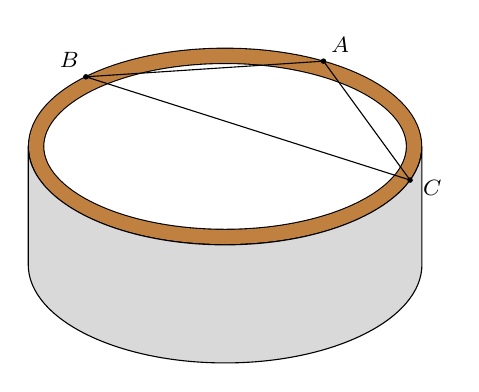
\begin{tikzpicture}[font=\footnotesize, line join=round, line cap=round, >=stealth, scale=1]
\def\bkl{2.5}\def\bkn{1.25}
\path (0,0) coordinate (O) (\bkl,0) coordinate (A) (-\bkl,0) coordinate (B);
\draw[double=brown, double distance=1.8mm, ] (O) ellipse ({\bkl-0.1} and {\bkn-0.1});
\draw[fill=gray!30] (A)--++(-90:1.5) arc (0:-180:{\bkl} and {\bkn})--(B) arc (180:360:{\bkl} and {\bkn});
\fill (60:{\bkl} and {\bkn}) circle (1pt)+(45:0.3)node{$A$}
(135:{\bkl} and {\bkn}) circle (1pt)+(135:0.3)node{$B$}
(-20:{\bkl} and {\bkn}) circle (1pt)+(-20:0.3)node{$C$};
\draw (60:{\bkl} and {\bkn})--(135:{\bkl} and {\bkn})--(-20:{\bkl} and {\bkn})--cycle;
\end{tikzpicture}
\end{center}
\choiceTF
	{\True Diện tích tam giác $ABC$ là $500$ cm$^2$}
	{Độ dài cạnh $BC$ là $80$ cm (kết quả được làm tròn đến hàng đơn vị)}
	{\True Bán kính miệng giếng là $87$ cm (kết quả được làm tròn đến hàng đơn vị)}
	{\True Chu vi miệng giếng bằng $546$ cm (kết quả làm tròn đến hàng đơn vị)}
\loigiai{
	\begin{itemchoice}
		\itemch Diện tích tam giác $ABC$ là $S=\dfrac{1}{2}\cdot AB \cdot AC \cdot \sin A=\dfrac{1}{2}\cdot 40 \cdot 50 \cdot \sin150^\circ = 500$ (cm$^2$).
		\itemch Áp dụng định lí côsin ta có
		\begin{eqnarray*}
			BC&=&\sqrt{AB^2+AC^2-2\cdot AB \cdot AC \cos A}=\sqrt{40^2+50^2-2\cdot40\cdot50\cos150^\circ}\\
			&=&\sqrt{4\,100+2\,000\sqrt3}\approx 87\ (\text{cm}).
		\end{eqnarray*}
		\itemch Áp dụng định lí sin ta có $\dfrac{BC}{\sin A}=2R$.\\
		Suy ra
		$$R=\dfrac{BC}{2\sin A}=\dfrac{\sqrt{4\,100+2\,000\sqrt3}}{2\sin 150^\circ}=\sqrt{4\,100+2\,000\sqrt3}\approx 87\ (\text{cm}).$$
		\itemch Chu vi miệng giếng là
		$$C=2\pi R = 2\pi \cdot \sqrt{4\,100+2\,000\sqrt3} \approx 546\ (\text{cm}).$$
	\end{itemchoice}
}
\end{ex}
\Closesolutionfile{ans}

\begin{center}
\textbf{PHẦN 3 - CÂU TRẮC NGHIỆM TRẢ LỜI NGẮN}% 4 câu 
\end{center}
\setcounter{ex}{0}
\Opensolutionfile{ans}[ans/ans-KQ-10-ONTAPCHUONG-IV-DE3]
\begin{ex}%[0H4H1-2]%[Dự án D - Đợt 4 NH24-25 - Lê Hữu Kiệt]
Giá trị của biểu thức $A = \sin120^\circ + 2\cos30^\circ - 3\sin45^\circ = \dfrac{\sqrt{a}-3\sqrt{b}}{2}$ với $a$; $b$ là các số nguyên dương. Khi đó giá trị $S = a+b^2$ bằng bao nhiêu?
\par\shortans{$7$}
\loigiai{
Ta có $A = \dfrac{\sqrt3}{2} + 2 \cdot \dfrac{\sqrt3}{2} - 3 \cdot \dfrac{\sqrt2}{2} = \dfrac{\sqrt3-3\sqrt2}{2}$.\\
Suy ra $a=3$ và $b=2$.\\
Vậy $S=a+b^2=3+2^2=7$.
}
\end{ex}

\begin{ex}%[0H4H2-1]%[Dự án D - Đợt 4 NH24-25 - Lê Hữu Kiệt]
Cho tam giác $ABC$ có $\dfrac{5}{\sin A}=\dfrac{4}{\sin B}=\dfrac{3}{\sin C}$ và $BC=10$ cm. Chu vi tam giác $ABC$ bằng bao nhiêu centimét?
\par\shortans{$24$}
\loigiai{
Theo định lí sin ta có $\dfrac{BC}{\sin A}=\dfrac{CA}{\sin B}=\dfrac{AB}{\sin C}$.\\
Suy ra $\dfrac{10}{\sin A}=\dfrac{CA}{\sin B}=\dfrac{AB}{\sin C}$.\\
Từ giả thiết $\dfrac{5}{\sin A}=\dfrac{4}{\sin B}=\dfrac{3}{\sin C}$, suy ra $\dfrac{10}{\sin A}=\dfrac{8}{\sin B}=\dfrac{6}{\sin C}$.\\
So sánh hai chuỗi tỉ lệ thức trên, ta suy ra $CA=8$ (cm) và $AB=6$ (cm).\\
Vậy chu vi tam giác $ABC$ bằng $BC+CA+AB=10+8+6=24$ (cm).
}
\end{ex}

\begin{ex}%[0H4V3-2]%[Dự án D - Đợt 4 NH24-25 - Lê Hữu Kiệt]
Từ một tấm bìa hình tròn bằng giấy, bạn Mai cắt ra một hình tam giác có các cạnh $AB=9$ cm, $AC=3\sqrt{13}$ cm và $\widehat{B}=60^\circ$ (xem hình bên dưới). Diện tích phần giấy còn lại của hình tròn (phần được tô xám) có diện tích bằng bao nhiêu centimét vuông (làm tròn kết quả đến hàng phần mười)?
\begin{center}
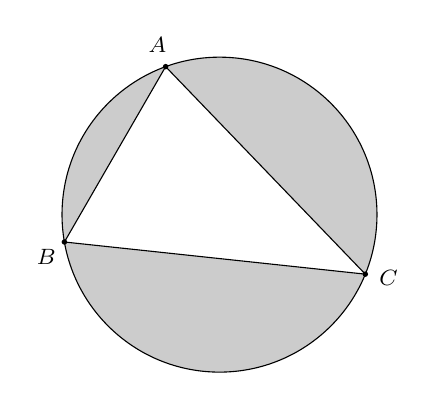
\begin{tikzpicture}[font=\footnotesize, line join=round, line cap=round, >=stealth, scale=1]
\def\bk{2}
\pgfmathsetmacro\gocA{asin(12/(2*sqrt(39)))}
\path (0,0) coordinate (O) (-170:\bk) coordinate (B) (110:\bk) coordinate (A)
(-170+2*\gocA:\bk) coordinate (C);
\draw[fill=gray!40] (O) circle (\bk);
\draw[fill=white] (A)--(B)--(C)--cycle;
\foreach \x/\g in {A/110, B/-140, C/-10}{\fill (\x) circle (1pt)+(\g:0.3)node{$\x$};}
\end{tikzpicture}
\end{center}
\par\shortans{$75{,}8$}
\loigiai{
Đặt $BC=x$ ($0< x < 9+3\sqrt{13}$).\\
Áp dụng định lí côsin ta có $AC^2 = AB^2 + BC^2 - 2 \cdot AB \cdot BC \cdot \cos B$.\\
Suy ra $117 = 81+x^2-2 \cdot 9 \cdot x \cos 60^\circ$, rút gọn ta được $x^2-9x-36=0$.\\
Giải phương trình ta được $x=-3$ hoặc $x=12$.\\
Do $0< x < 9+3\sqrt{13}$ ta nhận $x=12$. Suy ra $BC=12$ (cm).\\
Diện tích $\triangle ABC$ là $S_{\triangle ABC}=\dfrac{1}{2}\cdot AB \cdot BC \cdot \sin B = \dfrac{1}{2}\cdot9\cdot12\cdot\sin60^\circ=27\sqrt3$ (cm$^2$).\\
Áp dụng định lí sin ta có $\dfrac{AC}{\sin B}=2R$, với $R$ là bán kính đường tròn ngoại tiếp $\triangle ABC$.\\
Suy ra $R=\dfrac{AC}{2\sin B}=\dfrac{3\sqrt{13}}{2\sin60^\circ}=\sqrt{39}$ (cm).\\
Diện tích của tấm bìa là $S=\pi R^2=\pi\cdot\sqrt{39}^2=39\pi$ (cm$^2$).\\
Diện tích phần giấy còn lại là $S-S_{\triangle ABC}=39\pi-27\sqrt3\approx 75{,}8$ (cm$^2$).
}
\end{ex}

\begin{ex}%[0H4V3-2]%[Dự án D - Đợt 4 NH24-25 - Lê Hữu Kiệt]
Từ hai vị trí $A$ và $B$ của một tòa nhà, người ta quan sát đỉnh $C$ của ngọn núi. Biết rằng độ cao $AB$ bằng $70$ m, phương nhìn $AC$ tạo với phương nằm ngang góc $30^\circ$. Phương nhìn $BC$ tạo với phương nằm ngang góc $15^\circ 30'$. Chiều cao của ngọn núi so với mặt đất bằng bao nhiêu mét (không làm tròn các phép tính trung gian, làm tròn kết quả cuối cùng đến hàng đơn vị)?
\begin{center}
\begin{tikzpicture}[font=\footnotesize, line join=round, line cap=round, >=stealth, scale=0.7]
\path (0,0) coordinate (A) (0,3.5) coordinate (B) (11.7,0) coordinate (H)+(90:6.75) coordinate (C);
\begin{scope}
\clip (6.9,0) rectangle (13.1,6.78);
\draw[fill=gray!30]
	(7,0)
	.. controls +(80:1) and +(180:0.4) .. (9.5,4)
	.. controls +(10:1) and +(205:1) .. (C)
	.. controls +(-10:0.5) and +(110:0.4) .. (13,4.9)
	.. controls +(-90:2) and +(90:2) .. (13,0)
	;
\end{scope}
\draw[fill=gray!50] (A) rectangle +(-0.5,3.5);
\draw (A)--(C)--(B) (A)--(13,0)
	pic[draw, angle radius=2mm]{right angle=C--H--A};
\draw[dashed] (B)--++(11.7,0) (C)--(H);
\foreach \x/\g in {A/-90, B/90, C/90, H/-90}{\fill (\x) circle (10/7pt)+(\g:3/7)node{$\x$};}
\end{tikzpicture}
\end{center}
\par\shortans{$135$}
\loigiai{
Từ giả thiết suy ra $\triangle ABC$ có $\widehat{CAB}=60^\circ$; $\widehat{ABC}=105^\circ30'$ và $AB=70$.\\
Ta có $\widehat{ACB}=180^\circ-\widehat{CAB}-\widehat{ABC}=180^\circ-60^\circ-105^\circ30'=14^\circ30'$.\\
Áp dụng định lí sin ta có $\dfrac{AC}{\sin B}=\dfrac{AB}{\sin C}$, suy ra $AC=\dfrac{AB\sin B}{\sin C}=\dfrac{70\sin105^\circ30'}{\sin14^\circ30'}$.\\
Xét $\triangle ACH$ vuông tại $H$ ta có $\sin\widehat{CAH}=\dfrac{CH}{AC}$.\\
Suy ra $CH=AC\sin\widehat{CAH}=\dfrac{70\sin105^\circ30'}{\sin14^\circ30'}\cdot \sin30^\circ\approx 135$.\\
Vậy chiều cao của ngọn núi so với mặt đất là khoảng $135$ (m).
}
\end{ex}

\Closesolutionfile{ans}
\begin{center}
	\textbf{PHẦN 4 - TỰ LUẬN} % 3 câu
\end{center}
\setcounter{ex}{0}
\begin{ex}%[0H4H1-2]%[Dự án D - Đợt 4 NH24-25 - Lê Hữu Kiệt]
Tính trị biểu thức sau $D = \cos1^\circ + \cos2^\circ + \cos3^\circ + \cdots + \cos180^\circ$.
\loigiai{
Với $0\leq \alpha \leq 180^\circ$ ta có $\cos\alpha=-\cos(180^\circ-\alpha)$, suy ra $\cos\alpha+\cos(180^\circ-\alpha)=0$.
Khi đó
\begin{eqnarray*}
	D &=& (\cos1^\circ + \cos179^\circ) + (\cos2^\circ + \cos178^\circ) + \cdots + (\cos89^\circ + \cos91^\circ) + \cos90^\circ + \cos180^\circ\\
	&=& \left[\cos1^\circ + \cos(180^\circ - 1^\circ)\right] + \left[\cos2^\circ + \cos(180^\circ - 2^\circ)\right] + \cdots \\
	& &+ \left[\cos89^\circ + \cos(180^\circ - 89^\circ)\right] + \cos90^\circ + \cos180^\circ \\
	&=& 0 + 0 + \cdots + 0 + 0 + (- 1) \\
	&=& -1.
\end{eqnarray*}
Vậy $D=-1$.
}
\end{ex}

\begin{ex}%[0H4H2-1]%[Dự án D - Đợt 4 NH24-25 - Lê Hữu Kiệt]
Cho tam giác $ABC$ có $AB=3$, $AC=5$ và góc $\widehat{A}=120^\circ$. Gọi $M$ là trung điểm của cạnh $BC$. Tính độ dài đường trung tuyến $AM$.
\loigiai{
\begin{center}
\begin{tikzpicture}[font=\footnotesize, line join=round, line cap=round, >=stealth, scale=1]
\pgfmathsetmacro\gocB{acos(11/14)}
\path (0,0) coordinate (B) (7,0) coordinate (C) (\gocB:3) coordinate (A) ($(B)!1/2!(C)$) coordinate (M);
\draw (A)--(B)--(C)--cycle (A)--(M);
\foreach \x/\g in {A/90, B/-135, C/-45, M/-90}{\fill (\x) circle (1pt)+(\g:0.3)node{$\x$};}
\end{tikzpicture}
\end{center}
Áp dụng định lí côsin ta có $$BC=\sqrt{AB^2+AC^2-2\cdot AB\cdot AC\cdot \cos A}=\sqrt{3^2+5^2-2\cdot3\cdot5\cdot\cos120^\circ}=7.$$
Do $M$ là trung điểm của cạnh $BC$ nên $BM=\dfrac{BC}{2}=3{,}5$.\\
Áp dụng hệ quả định lí côsin ta có
$$\cos B=\dfrac{AB^2+BC^2-AC^2}{2\cdot AB \cdot BC}=\dfrac{11}{14}.$$
Xét $\triangle ABM$ ta có
$$AM=\sqrt{AB^2+BM^2-2\cdot AB\cdot BM\cdot\cos B}=\sqrt{3^2+3{,}5^2-2\cdot3\cdot3{,}5\cdot\dfrac{11}{14}}=\dfrac{\sqrt{19}}{2}.$$
Vậy $AM=\dfrac{\sqrt{19}}{2}$.
}
\end{ex}

\begin{ex}%[0H4V3-2]%[Dự án D - Đợt 4 NH24-25 - Lê Hữu Kiệt]
Chị Trang dùng một mảnh đất hình chữ nhật $ABCD$ để làm sân vườn như hình dưới. Chị dùng một phần đất là tứ giác $ABED$ để trồng hoa, phần còn lại chị lát gạch. Phần đất trồng hoa có các kích thước là $AB=15$ m, $BE=19$ m, $ED=10$ m, $DA=20$ m. Biết chi phí cho mỗi mét vuông trồng hoa là $300\,000$ đồng và mỗi mét vuông lát gạch là $250\,000$ đồng. Số tiền chị Trang cần có để làm sân vườn là bao nhiêu nghìn đồng (làm tròn kết quả đến hàng đơn vị)?
\begin{center}
\begin{tikzpicture}[font=\footnotesize, line join=round, line cap=round, >=stealth, scale=1]
\def\tile{2}
\path (0,0) coordinate (A)+(2*\tile,0) coordinate (D)
(0,1.5*\tile) coordinate (B)+(2*\tile,0) coordinate (C)
(1.4*\tile,1*\tile) coordinate (E);
\draw[pattern=dots] (A)--(B)--(E)--(D)--cycle;
\draw[pattern=bricks] (B)--(C)--(D)--(E)--cycle;
\fill (E) circle (1pt)+(45:0.4)node[circle, fill=white, inner sep=1]{$E$};
\foreach \x/\g in {A/-135, B/135, C/45, D/-45}{\fill (\x) circle (1pt)+(\g:0.4)node{$\x$};}
\end{tikzpicture}
\end{center}
\loigiai{
\begin{center}
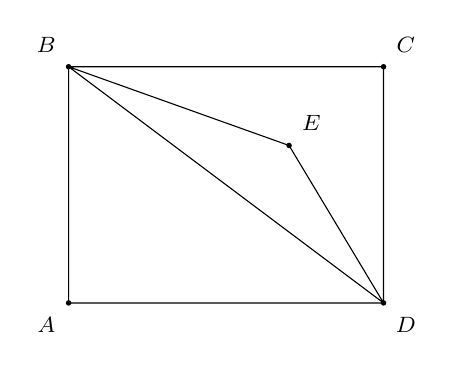
\begin{tikzpicture}[font=\footnotesize, line join=round, line cap=round, >=stealth, scale=1]
\def\tile{2}
\path (0,0) coordinate (A)+(2*\tile,0) coordinate (D)
(0,1.5*\tile) coordinate (B)+(2*\tile,0) coordinate (C)
(1.4*\tile,1*\tile) coordinate (E);
\draw (A)--(B)--(E)--(D)--cycle (B)--(D) (B)--(C)--(D)--(E)--cycle;
\fill (E) circle (1pt)+(45:0.4)node[circle, fill=white, inner sep=1]{$E$};
\foreach \x/\g in {A/-135, B/135, C/45, D/-45}{\fill (\x) circle (1pt)+(\g:0.4)node{$\x$};}
\end{tikzpicture}
\end{center}
Diện tích hình chữ nhật $ABCD$ là $S=AB\cdot AD=15\cdot20=300$ (m$^2$).\\
Xét $\triangle ABD$ vuông tại $D$, ta có
\begin{itemize}
	\item[] Diện tích tam giác $ABD$ là $S_{ABD}=\dfrac{1}{2}\cdot AB\cdot AD=\dfrac{1}{2}\cdot15\cdot20=150$ (m$^2$).
	\item[] Áp dụng định lí Pythagore ta có $BD=\sqrt{AB^2+AD^2}=\sqrt{15^2+20^2}=25$ (m).
\end{itemize}
Xét $\triangle BED$ ta có
\begin{itemize}
	\item[] Nửa chu vi $p=\dfrac{BD+BE+ED}{2}=\dfrac{25+19+10}{2}=27$ (m).
	\item[] Áp dụng công thức Heron, diện tích $\triangle BED$ là
	$$S_{BDE}=\sqrt{p(p-BD)(p-BE)(p-ED)}=\sqrt{27(27-25)(27-19)(27-10)}=12\sqrt{51}\ (\text{m}^2).$$
\end{itemize}
Suy ra diện tích tứ giác $ABED$ là $S_{ABED}=S_{ABD}+S_{BED}=150+12\sqrt{51}$ (m$^2$).\\
Diện tích tứ giác $BCDE$ là $S-S_{ABED}=300-\left(150+12\sqrt{51}\right)=150-12\sqrt{51}$ (m$^2$).\\
Vậy số tiền chị Trang cần có để làm sân vườn là
$$300\left(150+12\sqrt{51}\right)+200\left(150-12\sqrt{51}\right)\approx 83\,738\ (\text{nghìn đồng}).$$
}
\end{ex}

